\Gls{doe} is the Cerner application for placing orders within the laboratory. This application allows you to register patients, place orders, and add orders onto existing Accession numbers.


\newthought{Open \gls{doe}} by clicking the \appicon{doe} icon from the \gls{ab}.\sidenote{\checkref{ch:ab_addapp}{\refptch{part:ab}{ch:ab_addapp} }{Refer to the \textsc{App-Bar Procedure} } if you need help adding it.}

\section{Terms to know:}
\begin{quote}
\begin{description}
    \bolditem{Client Field} The location of the patient encounter. In most cases, it's best to leave this \textbf{blank}.
    \bolditem{Patient Identifier Field} The field used to search for patients.
    \bolditem{Orderable Field}  The field used to search for tests.
    \bolditem{Scratch Pad} A list of tests waiting to be ordered. Tests in the scratch pad can be removed, or edited before placing an order.\\
    \end{description}
\end{quote}


\noindent
\begin{tikzpicture}
\node [anchor=west] (pif) at (-2,3.7) {\scshape{Patient ID Field}};
\node [anchor=west] (cf) at (-2,5) {\scshape{Client Field}};
\node [anchor=west] (ord) at (-2,2.6) {\scshape{Orderable Field}};
\node [anchor=west] (sp) at (-2,1) {\scshape{Scratch Pad}};
\begin{scope}[xshift=1.5cm]
    \node[anchor=south west,inner sep=0] (image) at (0,0) {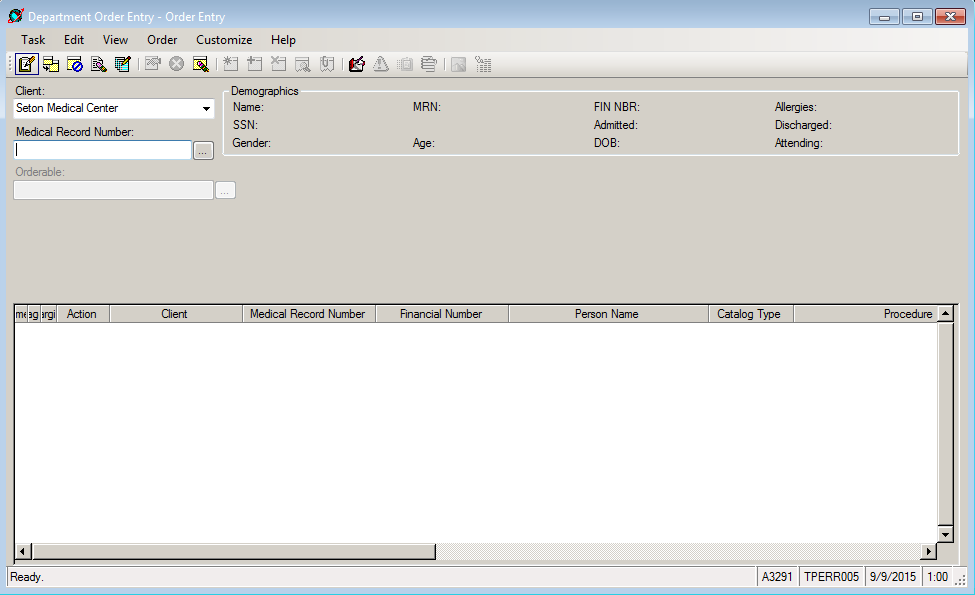
\includegraphics[width=0.7\textwidth]{graphics/doe_window}};
    \begin{scope}[x={(image.south east)},y={(image.north west)}]
        % \draw[amethyst,ultra thick,rounded corners] (0.01,0.73) rectangle (0.2,0.79);
        \draw [-stealth, line width=3pt, cyan500] (cf) to[out=0, in=-185] (0.01,0.82);
        \draw [-stealth, line width=3pt, deeporange500] (pif) to[out=0, in=-185] (0.01,0.75);
        \draw [-stealth, line width=3pt, indigo500] (ord) to[out=0, in=-145] (0.01,0.68);
        \draw [-stealth, line width=3pt, bluegrey500] (sp) to[out=0, in=-165] (0.01,0.2);
    \end{scope}
\end{scope}
\end{tikzpicture}%

